% see A1.4
\chapter{Planen}

Die Zeitplanung wird in der Abbildung \ref{fig:timeplan} oberhalb gezeigt. Die restlichen Aspekte der Planung sind in diesem Kapitel dokumentiert.

\begin{figure}[H]
  \begin{center}
    \begin{tikzpicture}
      \begin{umlsystem}[x=0, y=0]{PkOrg}
      \end{umlsystem}
      \umlactor[x=-5, y=.1]{Verantwortliche Fachperson}
      \umlactor[x=5, y=.1]{Hauptexperte}
      \umlassoc{Verantwortliche Fachperson}{PkOrg}
      \umlassoc{Hauptexperte}{PkOrg}
    \end{tikzpicture}
  \end{center}
  \caption[\enquote{Systemkontextdiagramm} erstellt mit Tikz UML]{Systemkontextdiagramm}
  \label{fig:systemcontext}
\end{figure}

\section{Diagramme}
In diesem Abschnitt werden verschiedene Diagramme, welche zur bildlichen Darstellung des Systems dienen sollen.
\subsection{Entity-Relationship-Diagram}
Das ERD zeigt die Beziehungen zwischen den einzelnen Entitäten. Da diese PA nur ein Plugin ist, welches neben
bereits bestehenden Entitäten seine eigenen erstellt, wird dort abgegrenzt. Nur Entitäten vom Plugin und
deren Beziehungen werden im ERD dargestellt. \newline
Hier werden zwei Optionen aufgezeigt und erklärt, welche im Kapitel \ref{chap:decide} (Entscheiden) ausgewertet werden. \newline
Die Attribute wurden auf Basis der Semaphore Webhooks Dokumentation \cite{semaphore_webhooks} und der GitHub Webhooks
Dokumentation über Pull Requests \cite{github_webhooks_pr} erstellt.

\begin{minipage}{\textwidth}
  \subsubsection{Option 1: Mehrere Entitäten}
  Die erste Option ist, dass für Deployments und Pull-Requests eigene Entitäten erstellt werden. Das würde wie folgt aussehen:
  \begin{center}
    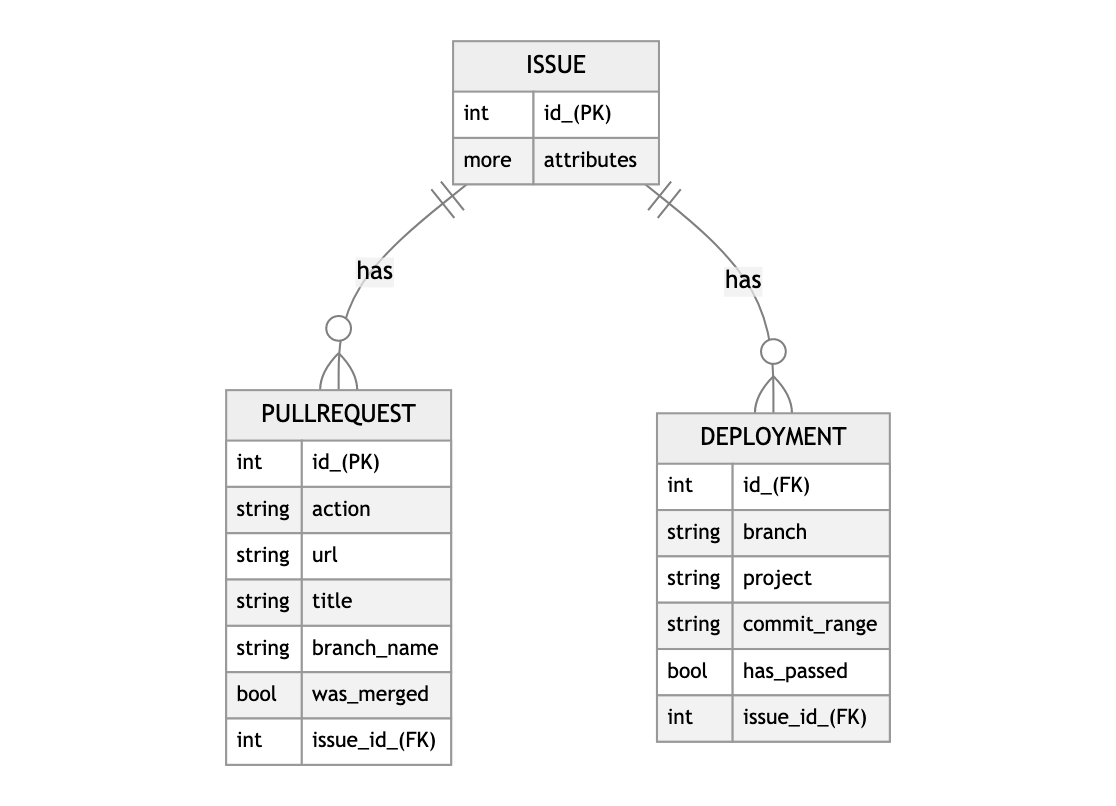
\includegraphics[width=0.8\textwidth]{images/erd/multiple.png}
    \label{fig:erd_multiple}
  \end{center}
\end{minipage}

\begin{minipage}{\textwidth}
  \subsubsection{Option 2: Inheritance}
  Die zweite Option ist, dass für Deployments und Pull-Requests keine eigenen Entitäten erstellt werden, sondern diese von
  einer gemeinsamen Entität erben. Das würde wie folgt aussehen:
  \begin{center}
    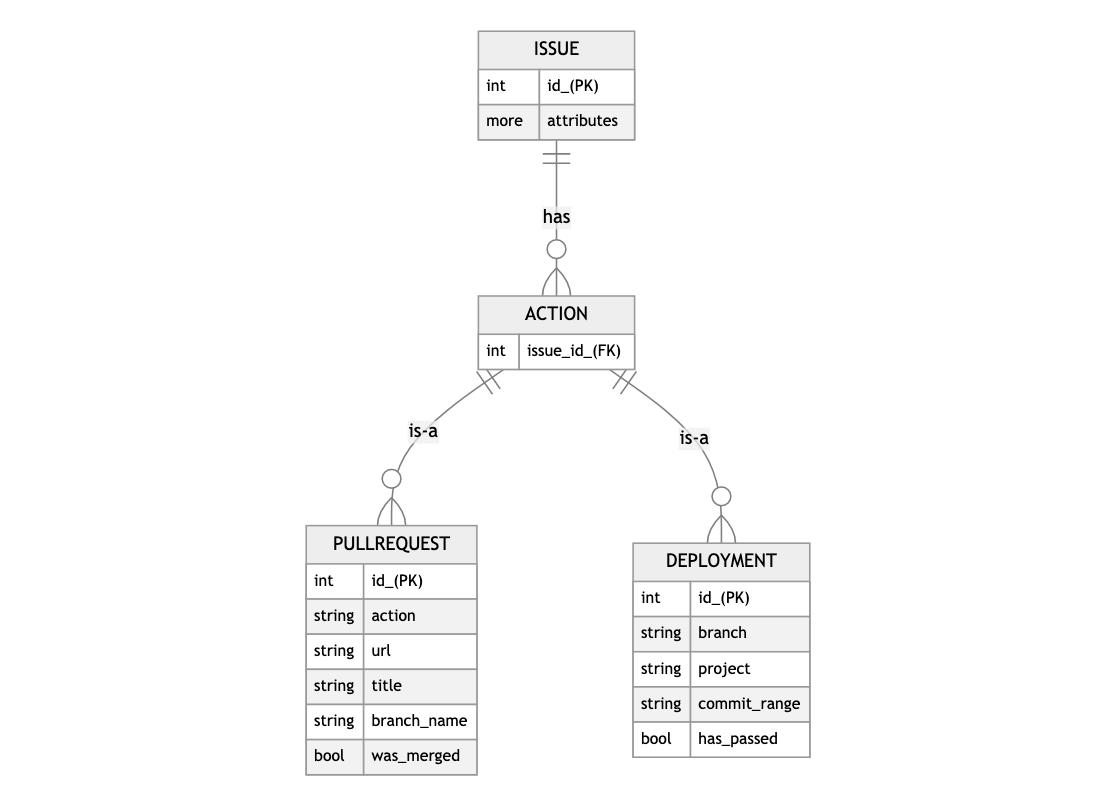
\includegraphics[width=0.8\textwidth]{images/erd/inheritance.png}
    \label{fig:erd_inheritance}
  \end{center}
\end{minipage}

\begin{minipage}{\textwidth}
  \subsection{Activity-Diagram}
  Das Activity-Diagramm zeigt den Ablauf des Plugins. In diesem Fall gibt es zwei Abläufe:
  \begin{itemize}
    \item Hook von SemaphoreCI oder GitHub
    \item Abfragen der Issues \newline
  \end{itemize}
\end{minipage}

\begin{minipage}{\textwidth}
  \subsubsection{Hook call}
  Die Hook calls werden von SemaphoreCI oder GitHub ausgelöst. Beide bei unterschiedlichen Events, welche beide mit Sanduhren
  dargestellt wurden:
  \begin{center}
    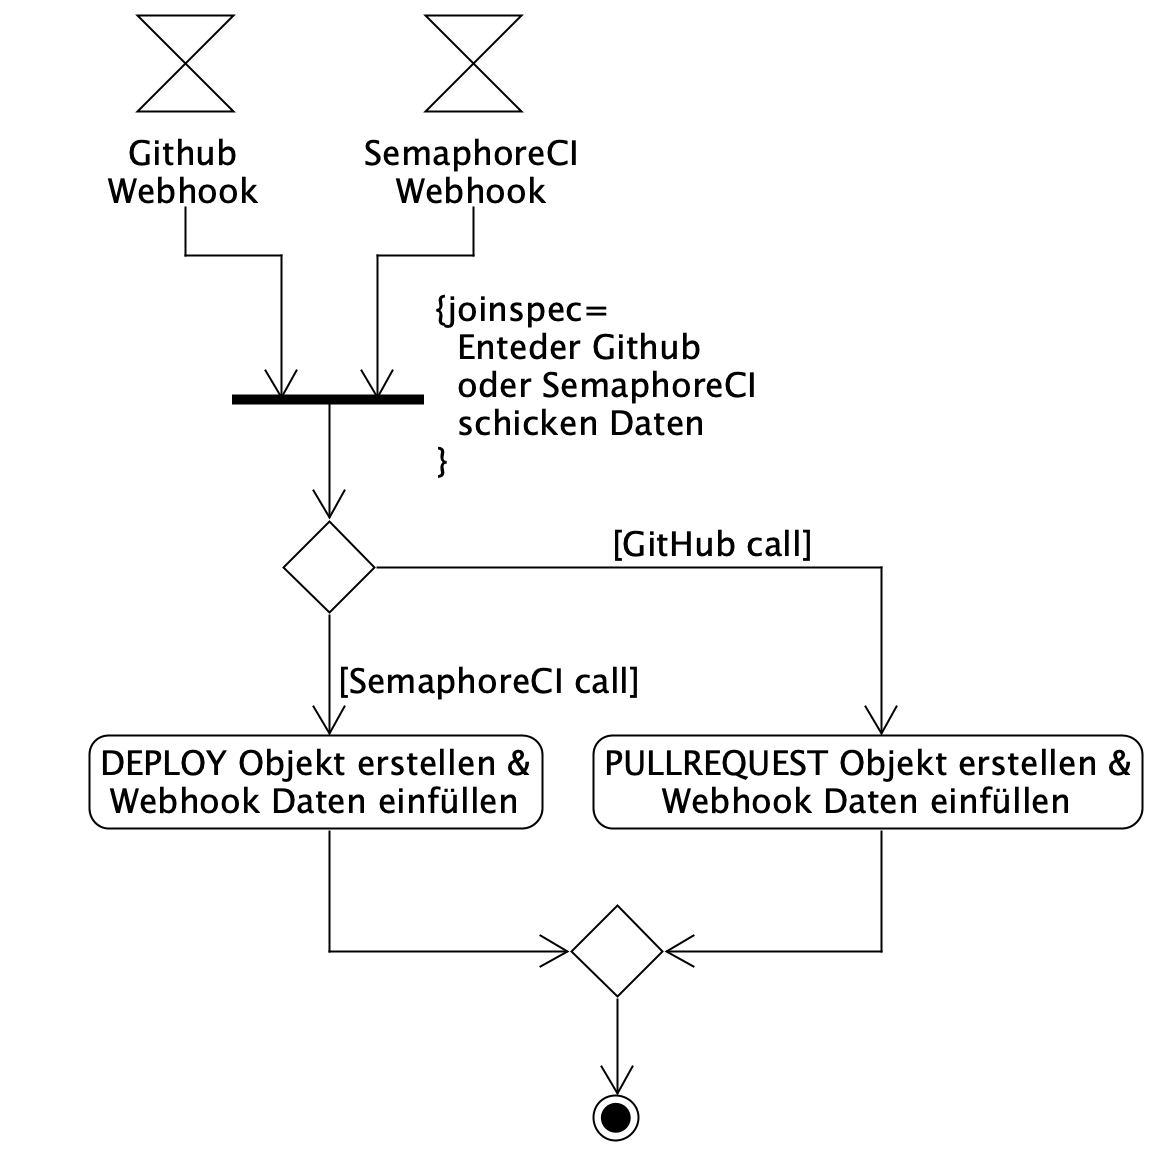
\includegraphics[width=0.8\textwidth]{images/activity/webhook.png}
    \label{fig:activity_hook_call}
  \end{center}
\end{minipage}

\begin{minipage}{\textwidth}
  \subsubsection{Abfrage der Issues}
  Falls der Nutzer auf die Details eines Issues klickt, wird eine Abfrage an das Plugin gesendet, welches die Pull Requests sowie
  Deployments abfragt und diese zurückgibt: \newline
  \begin{center}
    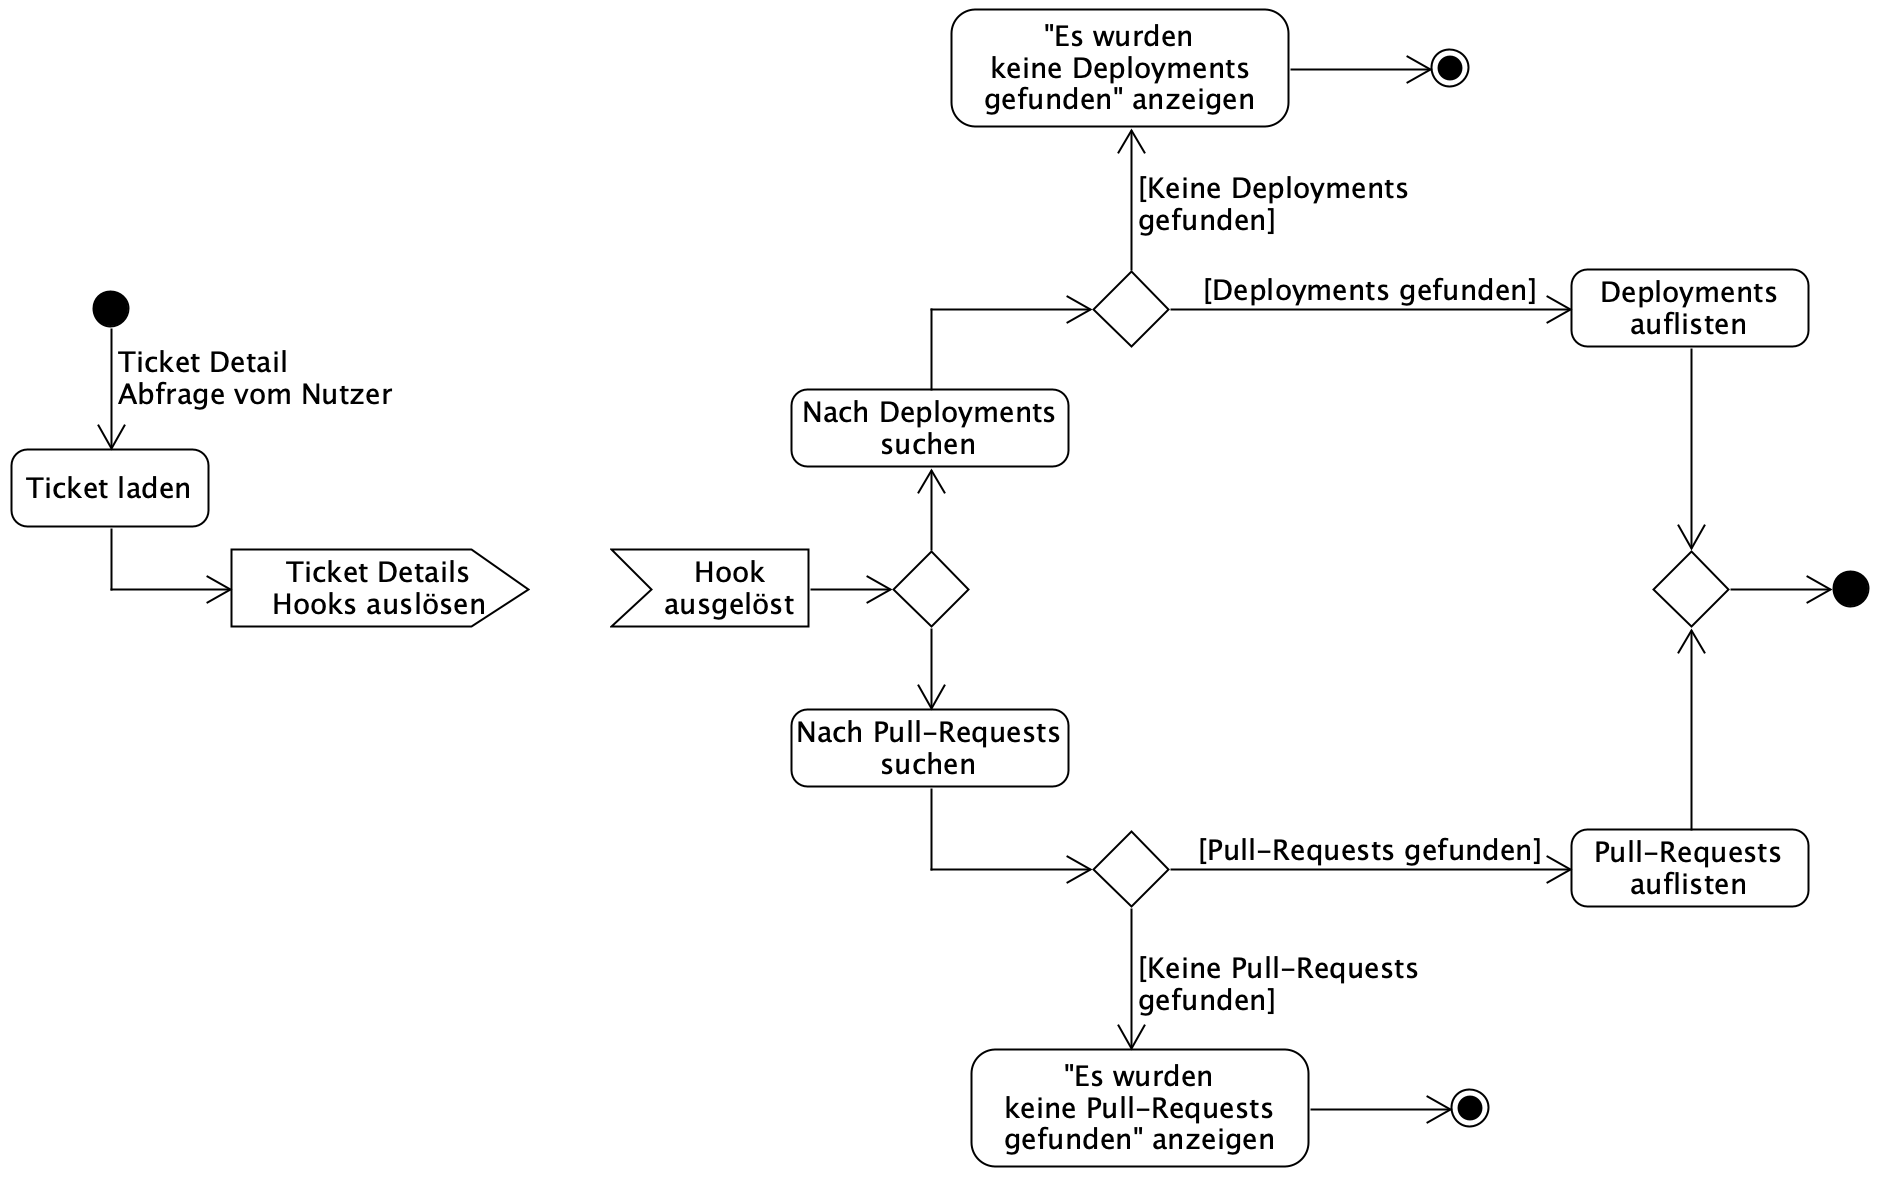
\includegraphics[width=0.8\textwidth]{images/activity/issues-view.png}
    \label{fig:activity_issues}
  \end{center}
\end{minipage}

\begin{minipage}{\textwidth}
  \subsection{Mockups}
  Damit die UI besser geplant werden kann, wird diese mit Mockups visualisiert. Diese Mockups sollen
  nur ungefähr wiedergeben, wie die UI aussehen soll. Da das Plugin auf einer bereits existierenden 
  Ansicht aufbaut, nämlich der Issue-View, wird diese nur sehr abstrahiert dargestellt. \newline
  Die bereits existierende Ansicht ist in der Abbildung mit weniger Opazität dargestellt. \newline
  \begin{center}
    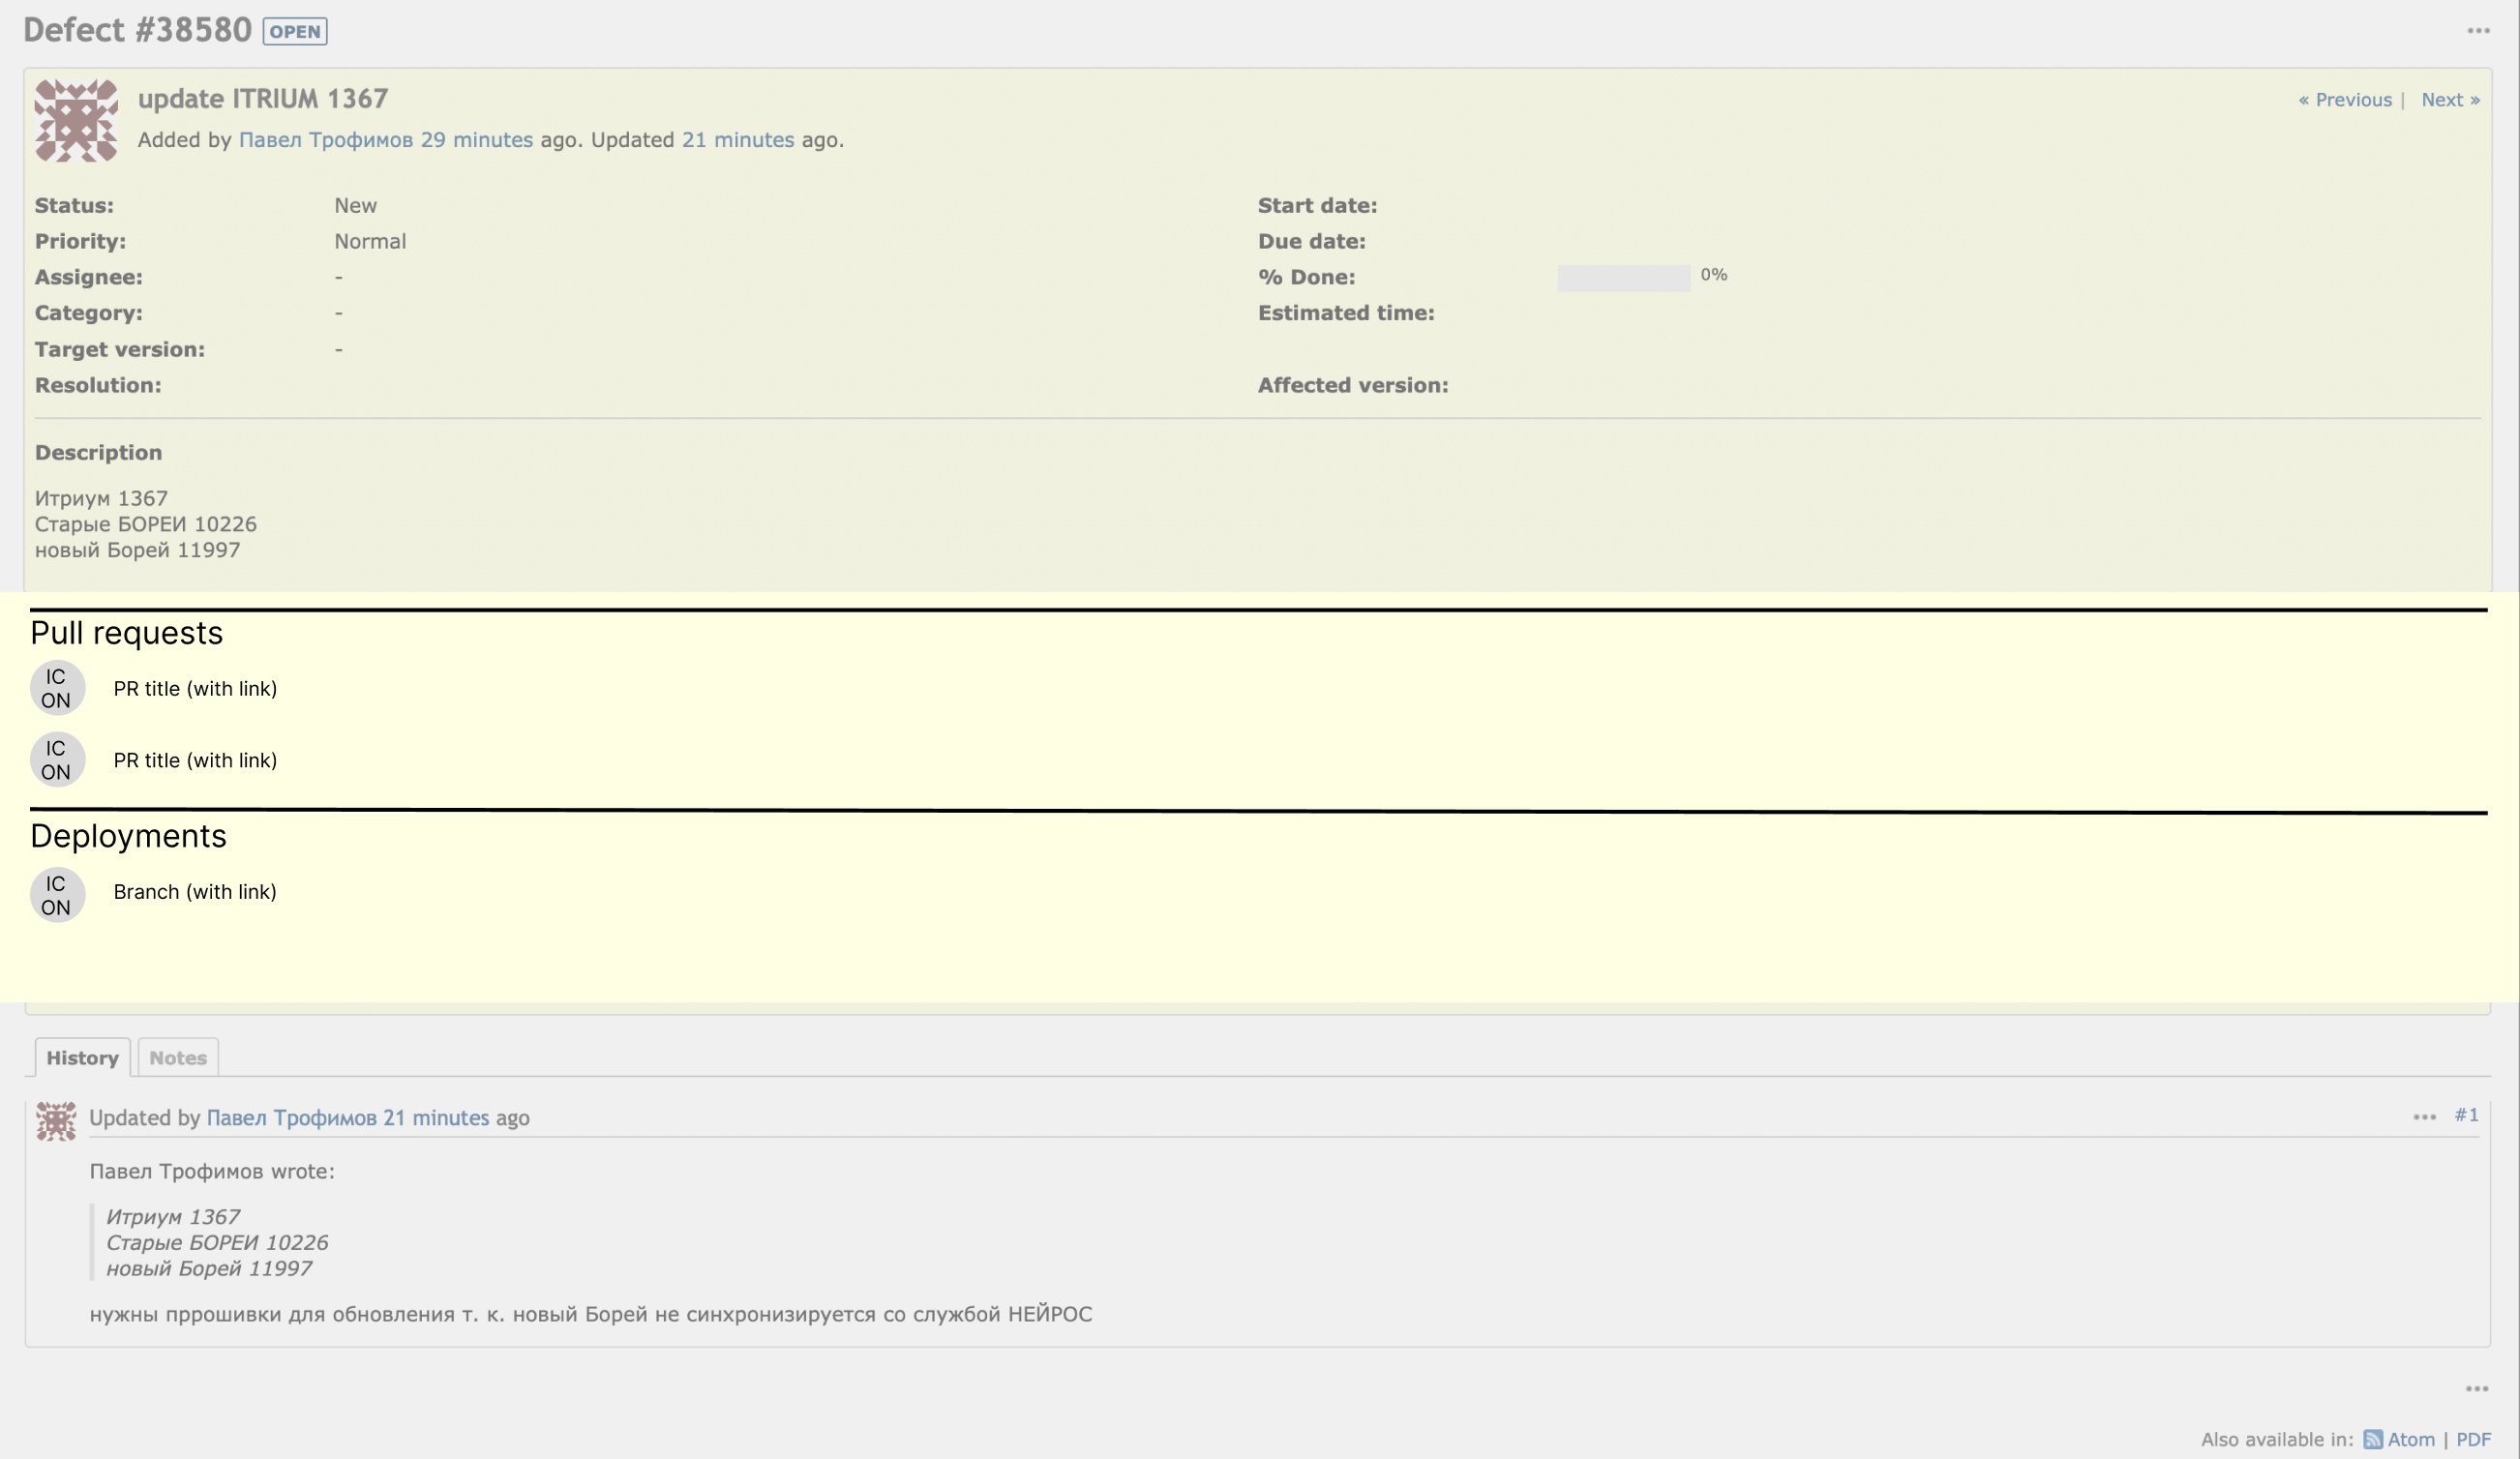
\includegraphics[width=0.8\textwidth]{images/mockup/details.png}
    \label{fig:mockup_details}
  \end{center}
\end{minipage}

\section{Testkonzept}
Das Testkonzept beschreibt, wie und mit welchen Werkzeugen das Resultat auf seine Richtigkeit kontrolliert wird.

\subsection{Automatisierte Tests}
Es werden automatisierte Tests für das Plugin geschrieben, welche die Funktionalität der Applikation testen.
Diese werden mit den gleichen Frameworks wie die vom Redmine geschrieben. Das heisst, dass die Tests mit
folgenden Frameworks geschrieben werden:
\begin{itemize}
  \item \textbf{MiniTest} für die Unit-Tests
  \item \textbf{Capybara} für die System-Tests
\end{itemize}
Die coverage sollte 100\% betragen (bei Klassen über 5 Zeilen). Diese Tests werden dann automatisch auf 
SemaphoreCI ausgeführt. Von der CI erhalten wir dann einen Coverage-Report, sowie eine Liste der
fehlgeschlagenen Tests. Nur falls alles in Ordnung ist, kann man die Pull-Request mergen.
\subsubsection{Weitere Tools}
Tools, welche nicht von Redmine selbst verwendet werden, welche aber dennoch im Plugin verwendet werden sind:
\begin{itemize}
  \item \textbf{Faker} für das Erstellen von realistischen Testdaten.
  \item \textbf{FactoryBot} für das Initialisieren von Objekten.
\end{itemize}
Die Coverage, sowie andere wichtige Informationen werden unter \ref{sec:automated-tests} dokumentiert.

\subsection{Manuelle Tests}
Während der Entwicklung und für allfällige Demonstrationszwecke werden manuelle Tests durchgeführt. Diese
werden in diesem Kapitel beschrieben und unter \ref{sec:manual-tests} protokolliert.

\begin{minipage}{\textwidth}
  \subsubsection{Verarbeiten von SemaphoreCI Daten}
  Um die Verarbeitung von SemaphoreCI Daten zu testen, gibt es zwei offensichtliche Möglichkeiten:
  \begin{itemize}
    \item \st{Senden von Daten per HTTP-Request an den lokalen Server}
    \item Benützen des Dienstes, damit dieser die Daten schickt
  \end{itemize}
  \textbf{Senden von Daten per HTTP-Request an den lokalen Server} \\
  Option eins ist das manuelle Senden von Daten an den lokalen Server. Dies kann man in der Konsole mit dem curl Programm
  \cite{everything_curl} machen. Dies ist jedoch eine sehr aufwändige und ungenaue Art zu testen, weshalb diese Option nicht
  weiter verfolgt wird. \newline

  \textbf{Benützen des Dienstes, damit dieser die Daten schickt} \\
  Die zweite Option ist, ein Repository auf GitHub zu erstellen und dieses mit SemaphoreCI zu verbinden. Es würde ein Deploy
  Script aufgesetzt werden, welches die SemaphoreCI Hooks auslöst. \newline
  Damit dann diese Daten beim lokalen Server ankommen können, müsste man mit ngrok \cite{ngrok_http_docs} einen HTTP Tunnel
  erstellen, welcher eine öffentliche IP zur Verfügung stellt. \newline
  Diese Methode ist auch sehr aufwändig, doch liefert genauere Daten als Option eins, weshalb diese benutzt wird. \newline
\end{minipage}

\begin{minipage}{\textwidth}
  \subsubsection{Verarbeiten von GitHub Daten}
  Auch die Verarbeitung der GitHub Daten kann man auf die gleiche Arten testen:
  \begin{itemize}
    \item \st{Senden von Daten per HTTP-Request an den lokalen Server}
    \item Benützen des Dienstes, damit dieser die Daten schickt \newline
  \end{itemize}
  \textbf{Senden von Daten per HTTP-Request an den lokalen Server} \\
  Die erste Option wird hier auch aus dem gleichen Grund wie bei SemaphoreCI nicht weiter verfolgt. \newline

  \textbf{Benützen des Dienstes, damit dieser die Daten schickt} \\
  Auch hier ist diese Option besser, da es zwar auch aufwändig ist, aber genauere Daten liefert. \newline
  Das Repository muss nicht mehr mit SemaphoreCI verbunden werden, doch gleich wie bei den SemaphoreCI Tests, müsse man
  mit ngrok \cite{ngrok_http_docs} einen HTTP Tunnel erstellen, welcher eine öffentliche IP zur Verfügung stellt.
\end{minipage}
\subsubsection{Der Nutzer schaut sich ein Ticket an mit Daten}
\subsubsection{Der Nutzer schaut sich ein Ticket an ohne Daten}

\subsection{Testmittel}
